\begin{figure}[h]
\centering
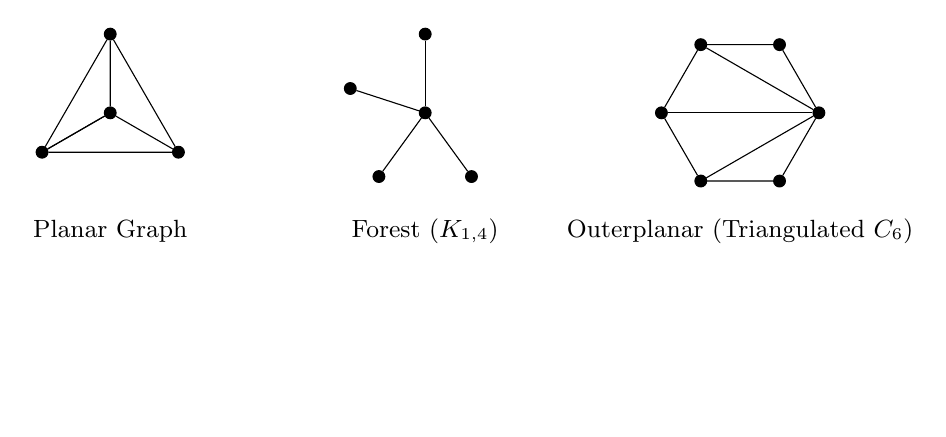
\begin{tikzpicture}[
    scale=1.0,
    every node/.style={circle,fill=black,draw,inner sep=1.5pt},
    baseline=(current bounding box.north)
]

% =============================
% 0. Planar Graph (simple triangulation)
% =============================
\begin{scope}[shift={(0,0)}]
\node (p1) at (90:1) {};
\node (p2) at (210:1) {};
\node (p3) at (330:1) {};

\node (p4) at (0,0) {};

\draw (p1)--(p2)--(p3)--(p1); % outer triangle
\draw (p1)--(p4)--(p2);
\draw (p2)--(p4)--(p3);

\node[draw=none,fill=none,yshift=-1.5cm] {\small Planar Graph};
\end{scope}

% =============================
% 1. Forest (Star K_{1,4})
% =============================
\begin{scope}[shift={(4,0)}]
\node (c) at (0,0) {};
\node (a1) at (90:1) {};
\node (a2) at (162:1) {};
\node (a3) at (234:1) {};
\node (a4) at (306:1) {};
\draw (c) -- (a1);
\draw (c) -- (a2);
\draw (c) -- (a3);
\draw (c) -- (a4);
\node[draw=none,fill=none,yshift=-1.5cm] {\small Forest ($K_{1,4}$)};
\end{scope}

% =============================
% 2. Outerplanar (Triangulated 6-cycle)
% =============================
\begin{scope}[shift={(8,0)}]
\node (b1) at (0:1) {};
\node (b2) at (60:1) {};
\node (b3) at (120:1) {};
\node (b4) at (180:1) {};
\node (b5) at (240:1) {};
\node (b6) at (300:1) {};

\draw (b1)--(b2)--(b3)--(b4)--(b5)--(b6)--(b1);

\draw (b1) -- (b3);
\draw (b1) -- (b4);
\draw (b1) -- (b5);

\node[draw=none,fill=none,yshift=-1.5cm] {\small Outerplanar (Triangulated $C_6$)};
\end{scope}
\end{tikzpicture}
\vspace{-5em} % tightly pulls caption up
\caption{Examples of Minor-Closed Families}
\end{figure}